\documentclass[12pt,twosides,onecolumn,openany]{article}
\usepackage{graphicx} 


\usepackage[catalan]{babel}
\usepackage{emptypage}
\usepackage{hyperref}
\usepackage{mathtools}
\usepackage{blindtext}
\usepackage{physics}
\usepackage{mhchem}
\usepackage[utf8]{inputenc}
\usepackage{caption}
\usepackage{subcaption}
\usepackage{wrapfig}
\usepackage[a4paper]{geometry}
\geometry{top=2.5cm, bottom=2.5cm, left=2.5cm, right=2.5cm}
\usepackage{fancyhdr}
\pagestyle{fancy}
\usepackage{amsmath}
\usepackage{amssymb}
\usepackage{amsfonts}
\providecommand{\norm}[1]{\lVert#1\rVert}
\hypersetup{colorlinks=true,urlcolor=blue,linkcolor=blue}
\usepackage{multirow}
\usepackage{multicol}
\usepackage{rotating}
\usepackage[backend=biber,style=numeric,sorting=none]{biblatex}

\usepackage{titlesec}

\newenvironment{Figura}
  {\par\medskip\noindent\minipage{\linewidth}}
  {\endminipage\par\medskip}

\titleformat{\section}  % comando de sección a formatear
  {\fontsize{14}{16}\bfseries} % formato para toda la línea
  {\thesection} % cómo mostrar el número
  {0.4em} % espacio entre el número y el texto
  {} % formato solo para el texto
  [] % formato para después del texto


\fancyhf{}
\fancyhead[LO,RE]{Grup D3}
\fancyhead[RO,LE]{Pràctica IIIa}
\fancyfoot[LO,RE]{\thepage}
\fancyfoot[RO,LE]{Laboratori de Termodinàmica - UAB}
\graphicspath{ {images/} }
\bibliography{pVa_referencies.bib}
\begin{document}
\begin{center}
    {\Large \textsc{Gasos reals: 
    Experiencia de Joule-Thompson}}\\
    \vspace{0.2cm}
    \textsc{28 d'Octubre de 2024\footnote{Pràctica realitzada originalment el 26 de Setembre de 2024.}}\\
    \vspace{0.2cm}
    \(\begin{matrix} 
    \text{Miguel A.} \hspace{1.5cm} & \text{Daniel B.} & \hspace{1.5cm} \text{Sergi R.}\\
    1637738 \hspace{1.5cm} & 1603508 & \hspace{1.5cm} 1607805
    \end{matrix}
    \)
\end{center}
\section{Introducció}
Aquesta pràctica té com a propòsit examinar com varia la temperatura del CO$_2$ quan aquest gas s'expandeix a través d'una barrera porosa, observant els canvis energètics associats. Per això, es calcula el coeficient de Joule-Thomson, que ajuda a determinar com el comportament del gas real difereix del d'un gas ideal, el qual no experimenta variacions energètiques durant l'expansió.\\\\
Amb l'ajuda del muntatge experimental descrit al document de pràctiques, es duran a terme diverses mesures. Primerament, mantenint constants $T_1$ i $P_1$ (temperatura i pressió del primer compartiment), es modificarà la pressió $P_2$ (amb $P_2 < P_1$) per crear un flux continu de gas i provocar l'expansió del CO$_2$. Les mesures es repetiran amb diferents valors de $P_2$ per traçar la corba $T-P$, el pendent de la qual permetrà calcular el coeficient de Joule-Thomson.\\\\
Posteriorment, fixant $P_2$ i variant $P_1$, s'obtindran corbes isoentàlpiques. Aquestes corbes són útils per identificar, en un ampli interval de temperatures, la corba d'inversió que delimita els punts on el coeficient de Joule-Thomson s'anul·la.\\\\
Finalment, es calcularà el coeficient de Joule-Thomson utilitzant les fórmules empíriques de Van der Waals \eqref{eq:vdw} i Beattie-Bridgman \eqref{eq:bb}, comparant els resultats teòrics amb els experimentals. Les expressions són:
\begin{equation}\label{eq:vdw}
\mu = \left( \frac{2a_v}{RT} \right) - \frac{b_v}{C_p}
\end{equation}
,
\begin{equation}\label{eq:bb}
\mu = \frac{1}{C_p} \left( -B_0 + \frac{2A_0}{RT} + \frac{4c}{T^3} + p \left( \frac{2B_0b}{RT} - \frac{3A_0a}{(RT)^2} + \frac{5B_0c}{RT^4} \right) \right)
\end{equation}
on $A_0$, $B_0$, $a$, $b$, $c$, $a_v$, $b_v$ són constants característiques del gas i $C_p$ és la capacitat calorífica molar.
\section{Resultats i discussió}
\subsection{Gràfiques $P-T$}
La Figura \ref{fig:1} mostra els resultats experimentals obtinguts, representant la temperatura en funció de la pressió. S'hi diferencien els estats inicials i finals, connectats per línies rectes que aproximen corbes isoentàlpiques.
\begin{figure}[h]
    \centering
    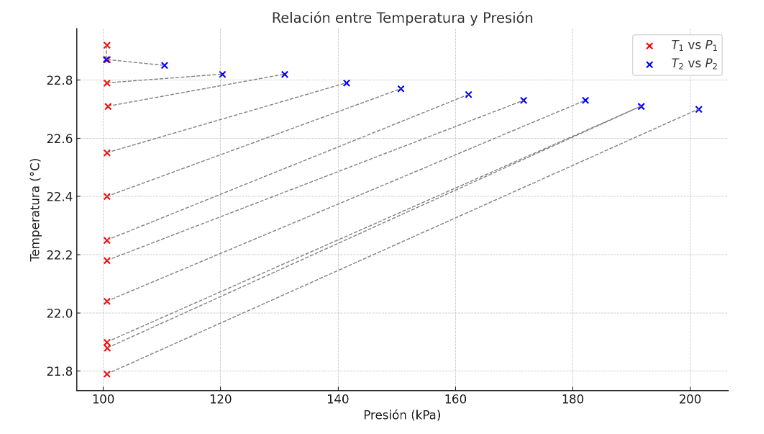
\includegraphics[width=0.85\linewidth]{../../reports/practica_IIIa/Captura2.PNG}
    \caption{Relació entre pressió i temperatura amb $P_1$ constant i $P_2$ variable.}
    \label{fig:1}
\end{figure}
\begin{figure}[h!]
    \centering
    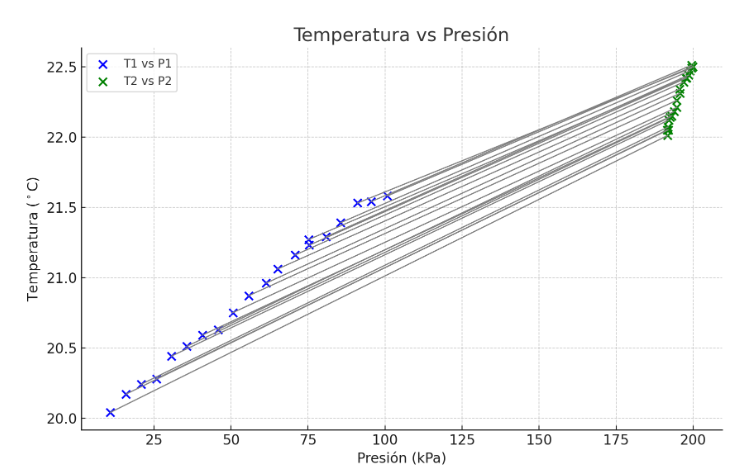
\includegraphics[width=0.85\linewidth]{../../reports/practica_IIIa/Captura.PNG}
    \caption{Relació entre pressió i temperatura amb $P_2$ constant i $P_1$ variable.}
    \label{fig:2}
\end{figure}
La Figura \ref{fig:2} presenta diverses corbes isoentàlpiques similars, on es podria calcular el coeficient de Joule-Thomson a partir del pendent de la recta tangent a cada corba.
\subsection{Determinació del coeficient de Joule-Thomson}
La Figura \ref{fig:3} mostra l'increment de temperatura en funció de l'increment de pressió. Els punts s'ajusten a una recta amb pendent $(134,3 \pm 1,8) \cdot 10^{-4}\,^\circ\text{C}/\text{kPa}$ i ordenada a l'origen $(0,598 \pm 0,047) ^\circ$C. Això proporciona un coeficient de Joule-Thomson:
\[
\mu = (134,3 \pm 1,8) \times 10^{-4} \ ^\circ\text{C}/\text{kPa} = (1,356 \pm 0,011) \ ^\circ\text{C}/\text{atm}
\]
\begin{figure}[h]
    \centering
    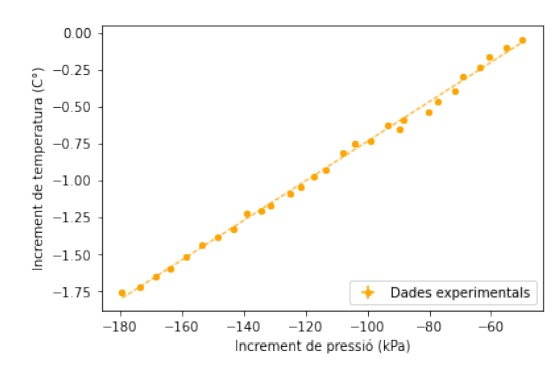
\includegraphics[width=0.85\linewidth]{../../reports/practica_IIIa/Captura3.PNG}
    \caption{Increment de temperatura respecte a l'increment de pressió.}
    \label{fig:3}
\end{figure}
\subsection{Comparació amb equacions empíriques}
Fent servir valors tabulats per al CO$_2$, l'equació de Van der Waals dóna $\mu = (0.693782 \pm 0.000047)$ K/atm, mentre que l'equació de Beattie-Bridgman resulta en $\mu = (1,18373 \pm 0,00038)\,\text{K}/\text{atm}$. Tot i les diferències, el model de Beattie-Bridgman és més adequat per a les condicions estudiades.
\section{Conclusions}
En aquesta pràctica, hem analitzat de manera quantitativa com el CO$_2$ s'allunya del comportament d'un gas ideal, calculant el coeficient de Joule-Thomson i examinant els canvis energètics que es produeixen durant l'expansió. Hem observat que el coeficient obtingut és positiu, la qual cosa indica que el gas es refreda en expandir-se, confirmant que no es comporta com un gas ideal.\\\\
A més, hem aproximat les corbes isoentàlpiques com a línies rectes, ja que el rang de pressions i temperatures utilitzat ho permetia. Aquestes dades, combinades amb les equacions empíriques, han mostrat que les temperatures estudiades estan molt allunyades de la temperatura d'inversió. Per tant, no ha estat possible derivar una expressió analítica per a les corbes isoentàlpiques a partir dels resultats obtinguts.
\section{Annexos}
Per a calcular la incertesa dels valors mesurats directament al laboratori s'ha fet servir la desviació estàndar de la mostra obtinguda de cada valor mesurat. Juntament amb la incertesa instrumental, calculem la incertesa de cada mesura com
\begin{equation*}
        u(x_i) = \sqrt{ s_{\text{est}}^2(x_i) + s_{\text{ins}}^2}
\end{equation*}
on $s_{\text{est}}$ és la desviació estàndar, $s_{\text{ins}}$ és la incertesa instrumental i $x_i$ és el valor mesurat.\\\\
Per a calcular la incertesa de magnituds derivades de les variables mesurades, s'ha fet servir la propagació d'incerteses, calculada com
\begin{equation*}
    u^2(y) = \sum_{i = 1}^{n} \left( \frac{\partial y}{\partial{x_i}} u(x_i)\right)^2
\end{equation*}
on $y$ és una funció tal que $y = y(x_1,...,x_n)$.
\subsection{Dades experimentals}
\renewcommand{\arraystretch}{1.65}
\begin{table}[h]
    \centering
    \caption{Dades preses en la variació de P2 cada aproximadament 10kPa}
    \label{tab:presstemp}
    \begin{tabular}{c|c|c|c}
        $T_1(^\circ \text{C})$ & $P_1(\text{kPa})$ & $T_2(^\circ \text{C})$ & $P_2(\text{kPa})$ \\
        \hline\hline
        21,79 $\pm$ 0,01 & 100,6 $\pm$ 0,1 & 22,70 $\pm$ 0,01 & 201,4 $\pm$ 0,1 \\
        21,88 $\pm$ 0,01 & 100,7 $\pm$ 0,1 & 22,71 $\pm$ 0,01 & 191,6 $\pm$ 0,1 \\
        21,90 $\pm$ 0,01 & 100,6 $\pm$ 0,1 & 22,71 $\pm$ 0,01 & 191,6 $\pm$ 0,1 \\
        22,04 $\pm$ 0,01 & 100,6 $\pm$ 0,1 & 22,73 $\pm$ 0,01 & 182,1 $\pm$ 0,1 \\
        22,18 $\pm$ 0,01 & 100,6 $\pm$ 0,1 & 22,73 $\pm$ 0,01 & 171,6 $\pm$ 0,1 \\
        22,25 $\pm$ 0,01 & 100,6 $\pm$ 0,1 & 22,75 $\pm$ 0,01 & 162,2 $\pm$ 0,1 \\
        22,40 $\pm$ 0,01 & 100,6 $\pm$ 0,1 & 22,77 $\pm$ 0,01 & 150,7 $\pm$ 0,1 \\
        22,55 $\pm$ 0,01 & 100,6 $\pm$ 0,1 & 22,79 $\pm$ 0,01 & 141,4 $\pm$ 0,1 \\
        22,71 $\pm$ 0,01 & 100,8 $\pm$ 0,1 & 22,82 $\pm$ 0,01 & 130,9 $\pm$ 0,1 \\
        22,79 $\pm$ 0,01 & 100,6 $\pm$ 0,1 & 22,82 $\pm$ 0,01 & 120,3 $\pm$ 0,1 \\
        22,87 $\pm$ 0,01 & 100,7 $\pm$ 0,1 & 22,85 $\pm$ 0,01 & 110,4 $\pm$ 0,1 \\
        22,92 $\pm$ 0,01 & 100,6 $\pm$ 0,1 & 22,87 $\pm$ 0,01 & 100,5 $\pm$ 0,1 \\
    \end{tabular}
\end{table}



\begin{table}[h]
    \centering
    \caption{Dades preses en la variació de P1 cada aproximadament 5kPa}
    \label{tab:presstemp}
    \begin{tabular}{c|c|c|c}

        $T_1(^\circ \text{C})$ & $P_1(\text{kPa})$ & $T_2(^\circ \text{C})$ & $P_2(\text{kPa})$ \\
        \hline\hline
        20,04 $\pm$ 0,01 & 10,8 $\pm$ 0,1 & 22,01 $\pm$ 0,01 & 191,7 $\pm$ 0,1 \\
        20,17 $\pm$ 0,01 & 15,89 $\pm$ 0,1 & 22,05 $\pm$ 0,01 & 191,6 $\pm$ 0,1 \\
        20,24 $\pm$ 0,01 & 20,8 $\pm$ 0,1 & 22,07 $\pm$ 0,01 & 191,8 $\pm$ 0,1 \\
        20,28 $\pm$ 0,01 & 25,8 $\pm$ 0,1 & 22,05 $\pm$ 0,01 & 191,9 $\pm$ 0,1 \\
        20,44 $\pm$ 0,01 & 30,6 $\pm$ 0,1 & 22,12 $\pm$ 0,01 & 192,1 $\pm$ 0,1 \\
        20,51 $\pm$ 0,01 & 35,6 $\pm$ 0,1 & 22,14 $\pm$ 0,01 & 192,5 $\pm$ 0,1 \\
        20,59 $\pm$ 0,01 & 40,7 $\pm$ 0,1 & 22,15 $\pm$ 0,01 & 193,1 $\pm$ 0,1 \\
        20,63 $\pm$ 0,01 & 45,8 $\pm$ 0,1 & 22,18 $\pm$ 0,01 & 193,8 $\pm$ 0,1 \\
        20,75 $\pm$ 0,01 & 50,6 $\pm$ 0,1 & 22,21 $\pm$ 0,01 & 194,7 $\pm$ 0,1 \\
        20,87 $\pm$ 0,01 & 55,7 $\pm$ 0,1 & 22,26 $\pm$ 0,01 & 194,7 $\pm$ 0,1 \\
        20,96 $\pm$ 0,01 & 61,4 $\pm$ 0,1 & 22,31 $\pm$ 0,01 & 195,7 $\pm$ 0,1 \\
        21,06 $\pm$ 0,01 & 65,1 $\pm$ 0,1 & 22,34 $\pm$ 0,01 & 195,6 $\pm$ 0,1 \\
        21,16 $\pm$ 0,01 & 70,8 $\pm$ 0,1 & 22,39 $\pm$ 0,01 & 196,9 $\pm$ 0,1 \\
        21,23 $\pm$ 0,01 & 75,4 $\pm$ 0,1 & 22,42 $\pm$ 0,01 & 197,9 $\pm$ 0,1 \\
        21,27 $\pm$ 0,01 & 75,2 $\pm$ 0,1 & 22,42 $\pm$ 0,01 & 197,6 $\pm$ 0,1 \\
        21,29 $\pm$ 0,01 & 80,9 $\pm$ 0,1 & 22,44 $\pm$ 0,01 & 198,6 $\pm$ 0,1 \\
        21,39 $\pm$ 0,01 & 85,6 $\pm$ 0,1 & 22,47 $\pm$ 0,01 & 198,9 $\pm$ 0,1 \\
        21,53 $\pm$ 0,01 & 91,1 $\pm$ 0,1 & 22,49 $\pm$ 0,01 & 199,5 $\pm$ 0,1 \\
        21,54 $\pm$ 0,01 & 95,5 $\pm$ 0,1 & 22,51 $\pm$ 0,01 & 199,5 $\pm$ 0,1 \\
        21,58 $\pm$ 0,01 & 100,7 $\pm$ 0,1 & 22,50 $\pm$ 0,01 & 199,9 $\pm$ 0,1 \\

    \end{tabular}
\end{table}
















































\end{document}
